\chapter{Recherches}

\label{Chapter2}

\section{Formats de fichiers 3D}

\subsection{glTF}
https://www.khronos.org/gltf/

\section{Building Information Modeling (BIM)}

\begin{figure}
    \centering
    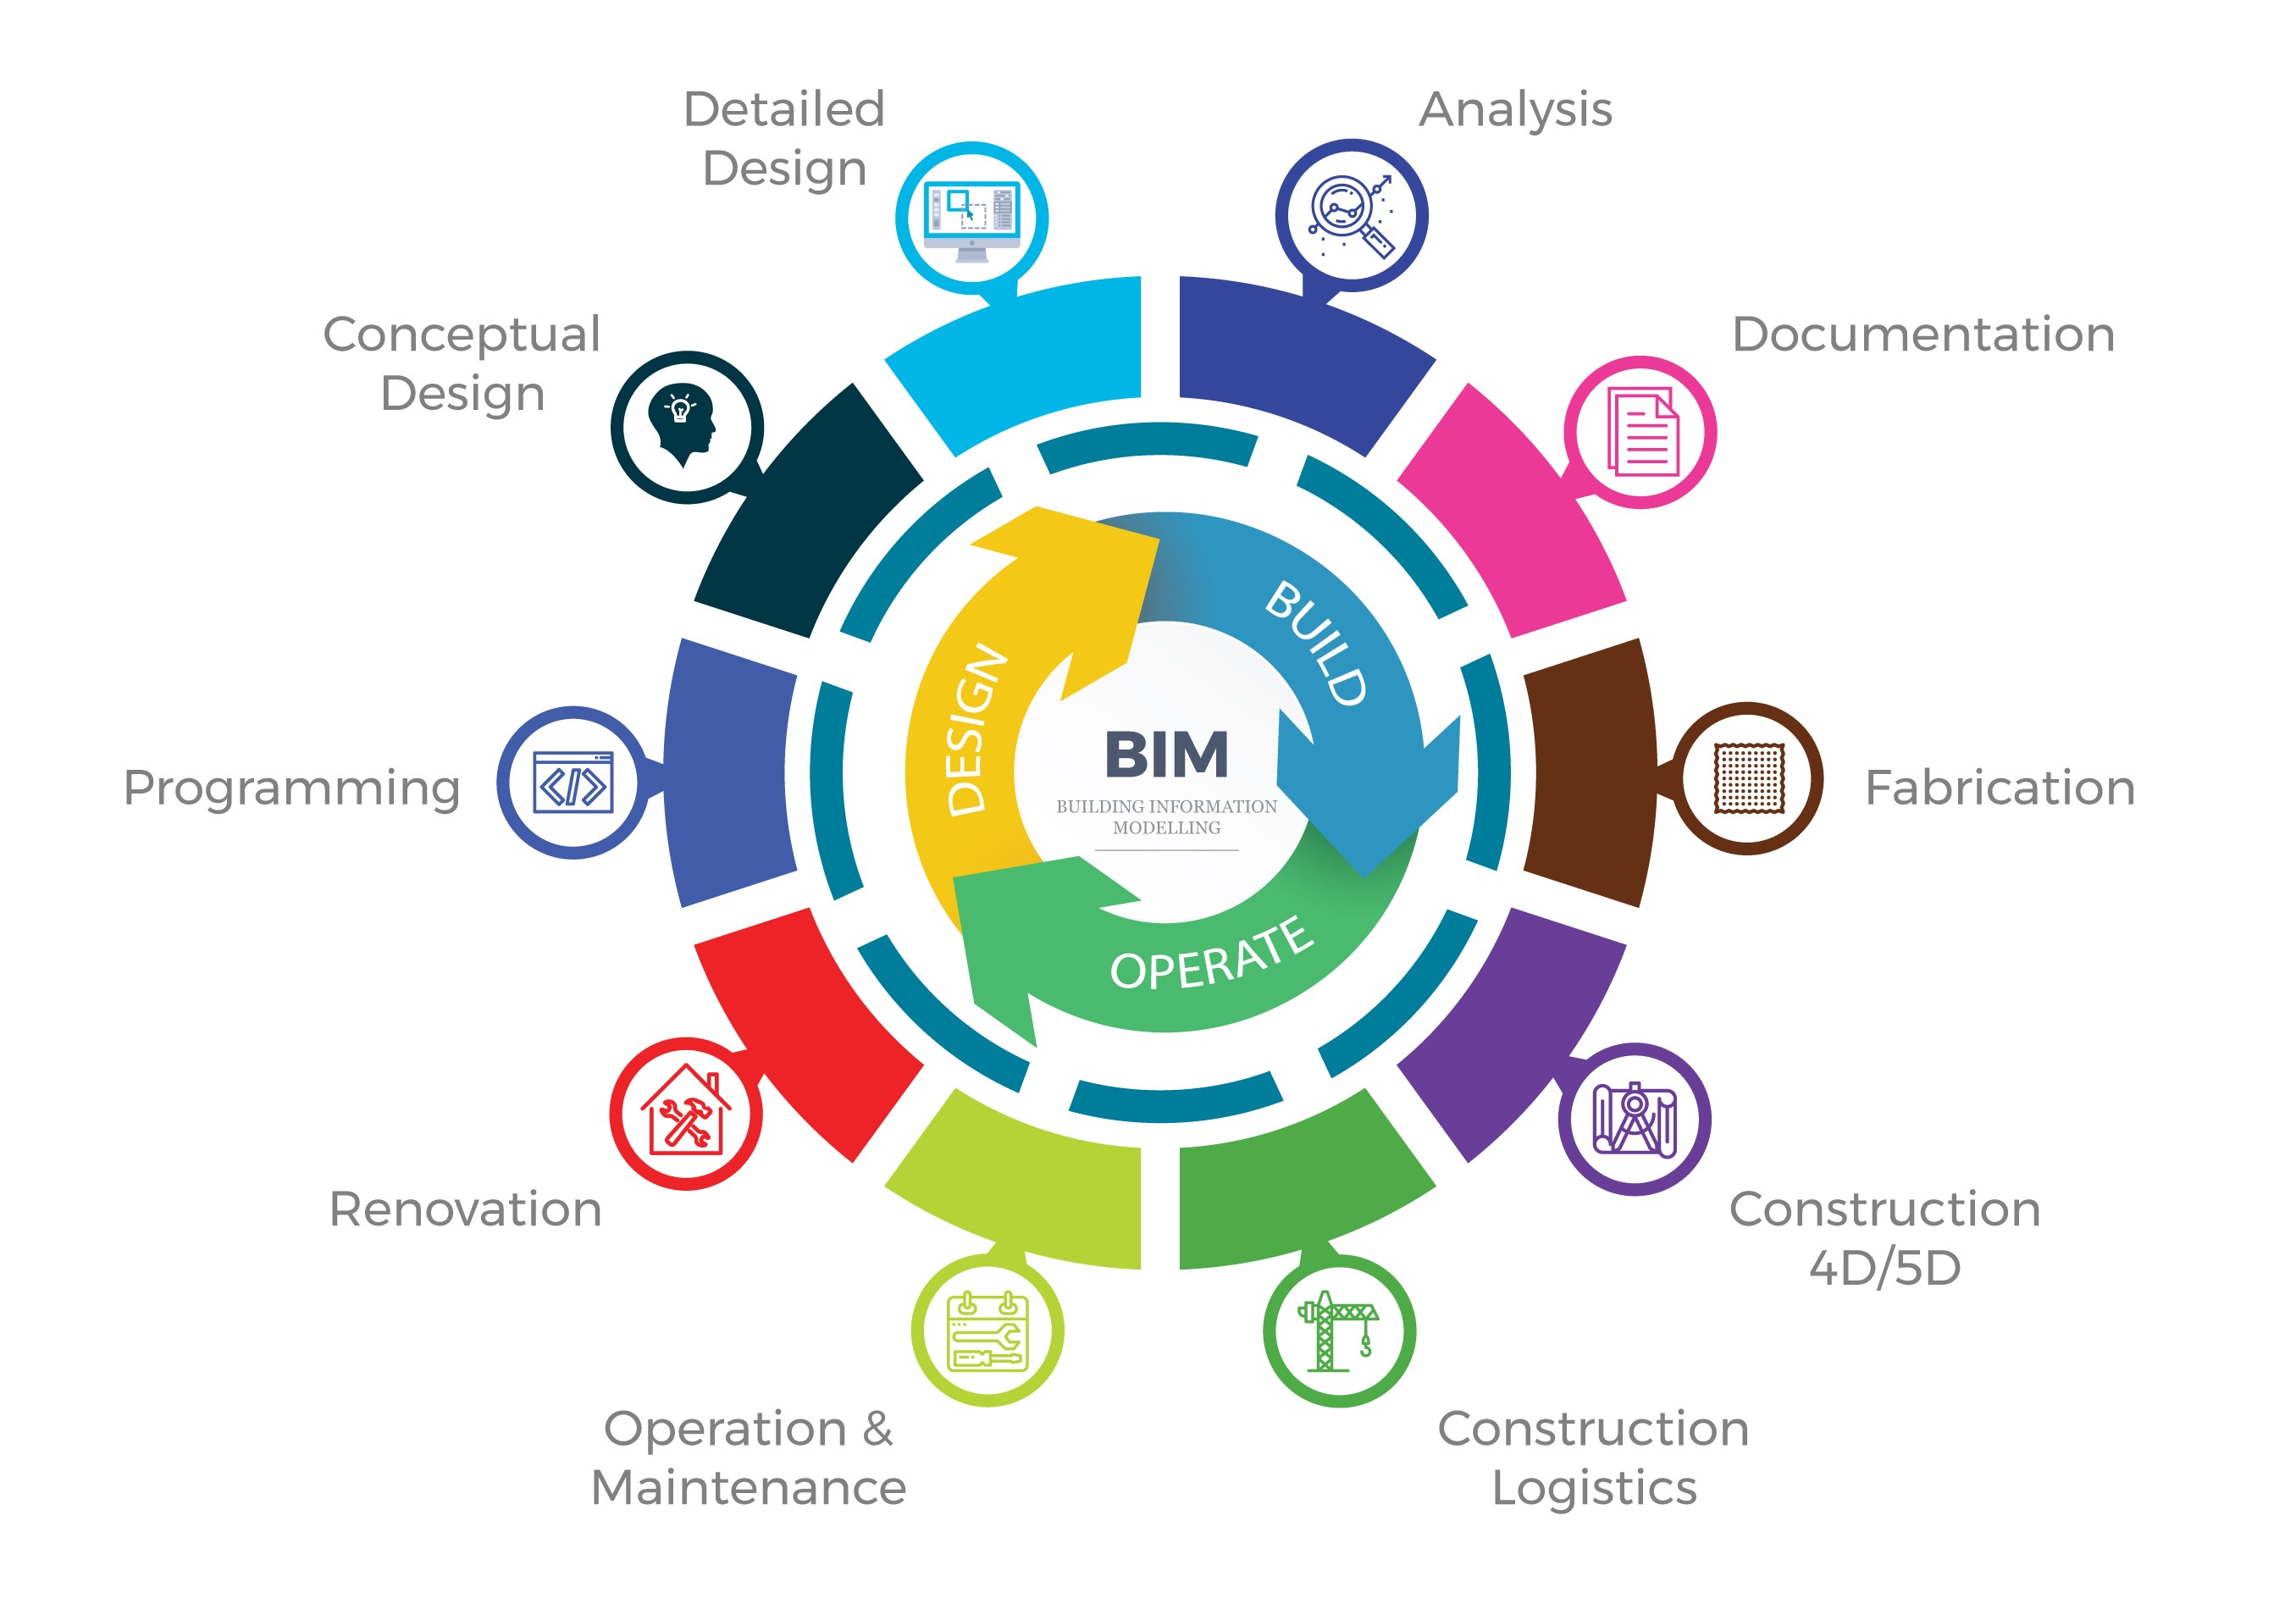
\includegraphics[width=\linewidth]{Figures/bim-process.jpg}
    \caption{Processus BIM}
    \label{fig:bim-process}
\end{figure}

\url{http://objectif-bim.com/index.php/openbim/bcf-format-de-collaboration-bim}
\url{http://njhcadservices.co.uk/?page_id=32}

\section{Cas d'utilisation}

\begin{figure}
    \centering
    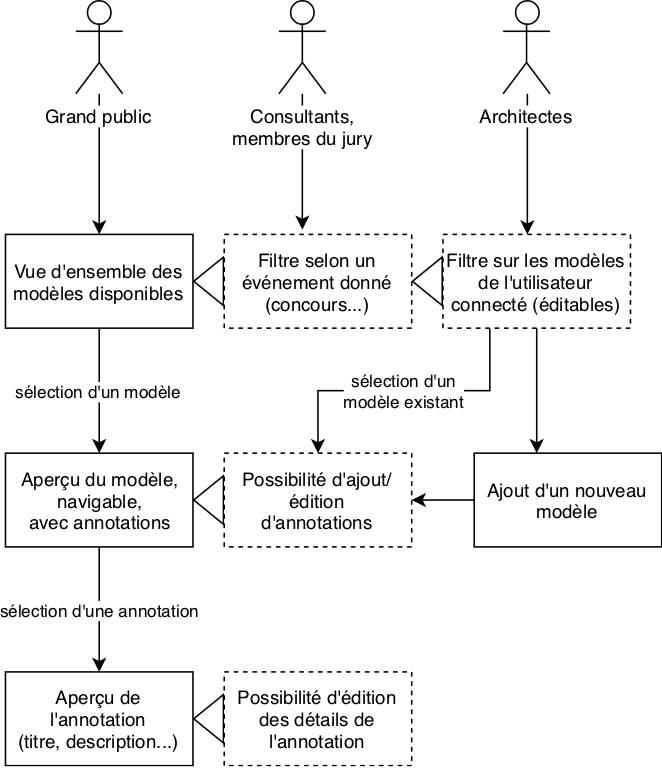
\includegraphics[width=\linewidth]{Figures/use-cases.png}
    \caption{Exemples de cas d'utilisation}
    \label{fig:use-cases}
\end{figure}

\section{Visionneuse de modèles 3D}

L'affichage et la manipulation de modèles 3D constitue la première brique d'un tel projet, la fondation sur laquelle viendront s'ajouter les modules complémentaires souhaités, tels que la création d'annotations, le stockage des modèles et des notes associées, etc.
Il existe de multiples visionneuses, qu'elles soient en ligne ou à installer. Le choix se réduit lorsque l'on recherche des projets open-source, ce qui était nécessaire de le cadre de ce projet : autant partir sur une base existante, et ne pas réinventer la roue.

https://github.com/bwasty/gltf-viewer : glTF 2.0 Viewer written in Rust. Pas retenue, n'ayant aucune expérience en Rust

Le choix s'est porté sur three-gltf-viewer.
Il s'agit d'un projet développé par un gars de chez Google, spécialisé dans...,  apparemment dans son temps libre.
Le projet a été démarré récemment (DATE) et est encore actif - à l'heure où ces lignes sont écrites, le dernier \textit{commit} date du 16 avril. Cela conforte dans l'idée que les technologies utilisées pour le concevoir soient modernes.

Les spécificités de ce projet sont détaillées sous "Langages et technologies".


\section{Langages et technologies}

Lorsque l'on se base sur un projet existant, l'une des contraintes et qu'il va falloir s'adapter aux technologies employées par celui-ci.

Un rapide tour d'horizon sur la page Github du projet, en activant l'affichage de la proportion d'utilisation de langages, nous apprend qu'il s'agit d'un projet web, composé essentiellement de JavaScript.

\begin{figure}[h]
    \centering
    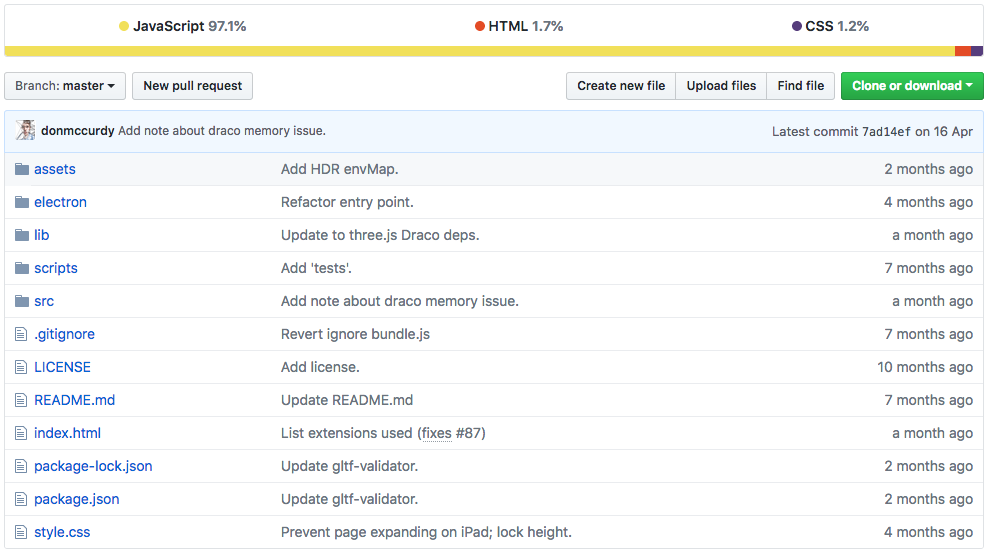
\includegraphics[width=\linewidth]{Figures/three-gltf-viewer-github-preview.png}
    \caption{Statistiquesdu projet three-gltf-viewer}
    \label{fig:three-gltf-viewer-github-preview}
\end{figure}

Les répertoires situées à la racine nous apprennent l'utilisation du framework Electron https://electronjs.org/.
Détailler ELECTRON

Package.json -> Node...

Migration JS -> TS : https://www.typescriptlang.org/docs/handbook/migrating-from-javascript.html
malheureusement prendrai trop de temps dans le cadre de ce projet. On peut mixer du TS dans du JS mais c'est pas très simple...
Guide pour migrer une app React vers TS : https://github.com/Microsoft/TypeScript-React-Conversion-Guide#typescript-react-conversion-guide

Javascript : cours J-L Falcone https://gitlab.unige.ch/courses/jsHepia


\section{Annotations}

Décrire les annotations proposées par Sketchfab : a un titre et une description. Peut aussi être une image.
Principe : en mode édition, double-clic à l'endroit souhaité (point 3d). pour ajouter une annotation. Celle-ci reste liée à la coordonnée choisie, et suit les mouvements appliqués au modèle 3D (p.ex. si on pivote le modèle, alors l'annotation effectue la même transformation).

Choix de technologie :. En gros, on pourrait tout faire en WebGL (REF sur doc WebGL), mais HTML/CSS est bien mieux adapté aux layouts/polices (voir explication en introduction de https://manu.ninja/webgl-three-js-annotations).

\section{Stockage}
Stockage des modèles 3D :

Stockage des annotations :

\section{Déploiement en continu avec Heroku}

Heroku considère que l'application se trouve à la racine du dossier.
Si l'application est située dans un sous-répertoire, l'une des possibilités est d'utiliser le module 'subtree' de git, qui permet de créer une sous-arborescence au sein d'un même projet. Ce dernier pourra alors être lié à une branche distincte, dans laquelle il se trouvera à la racine.
\begin{minted}{bash}
    git subtree push --prefix mysubtree origin subtree
\end{minted}

git subtree push --prefix mip-viewer origin heroku

Heroku est un environnement de production (pas de dev). Voir problème rencontré ici :

et commentaire :
Heroku is a production environment. The devDependencies are for packages that are required on your development environment only. Packages that you need to be included in your Heroku slug (including packages required during the slug build phase, such as webpack), need to be in your dependencies, not devDependencies. It is possible that you see people putting webpack in devDependencies for other platforms, but probably not for Heroku. 

et une possible solution étant de créer un script spécifique à Heroku : https://stackoverflow.com/a/42237745/1975002
Avantage : permet de ne pas faire grandir package.json, et d'isoler ce qui concerne Heroku.

Dans mon cas, comme seul le package 'webpack' était concerné, je l'ai "dédoublé" sous dependencies comme suggéré ici : https://stackoverflow.com/a/41973881/1975002

Heroku a pu ainsi faire une première build réussie de l'application. Celle-ci ne fonctionnait malheureusement pas encore correctement (voir https://github.com/MichaelPolla/mip-viewer/issues/5#issuecomment-390479224) 